\documentclass[11.5pt]{sig-alternate} % sets document style to sig-alternate
% packages
% typesetting
%\usepackage{dirtytalk} % typset quotations easier (\say{stuff})
\usepackage{hanging} % hanging paragraphs
\usepackage[defaultlines=3,all]{nowidow} % avoid widows
\usepackage[pdfpagelabels=false]{hyperref} % produce hypertext links, includes backref and nameref
\usepackage{xurl} % defines url linebreaks, loads url package
\usepackage{microtype}
%\usepackage[super]{nth} % easily create superscript ordinal numbers with \nth{x}
\usepackage{textgreek}
% layout
\usepackage{enumitem} % control layout of itemize, enumerate, description
\usepackage{fancyhdr} % control page headers and footers
\usepackage{float} % improved interface for floating objects
\usepackage{subcaption}
%\usepackage{multicol} % intermix single and multiple column pages
% language
\usepackage[utf8]{inputenc} % accept different input encodings
\usepackage[english]{babel} % multilanguage support
% misc
\usepackage{graphicx} % builds upon graphics package, \includegraphics
%\usepackage{lastpage} % reference number of pages
%\usepackage{comment} % exclude portions of text (?)
\usepackage{xcolor} % color extensions
\usepackage[backend=biber, style=apa]{biblatex} % sophisticated bibliographies % necessary for HTML to display author info and date on abstract page
\usepackage{csquotes} % advanced quotations, makes biblatex happy
\usepackage{authblk} % support for footnote style author/affiliation
% tables and figures
\usepackage{tabularray}
\UseTblrLibrary{varwidth}
%\usepackage{array} % extend array and tabular environments
\usepackage{caption} % customize captions in figures and tables (rotating captions, sideways captions, etc)
%\usepackage{cuted} % allow mixing of \onecolumn and \twocolumn on same page
\usepackage{multirow} % create tabular cells spanning multiple rows
%\usepackage{subfigure} % deprecated, support for manipulation of small figures
%\usepackage{tabularx} % extension of tabular with column designator "x", creates paragraph-like column whose width automatically expands
%\usepackage{wrapfig} % allows figures or tables to have text wrapped around them
%\usepackage{booktabs} % better rules
% dummy text
%\usepackage{blindtext} % blind text dummy text
%\usepackage{kantlipsum} % Kant style dummy text
\usepackage{lipsum} %lorem ipsum dummy text
% other helpful packages may be booktabs, longtable, longtabu, microtype

\pagestyle{fancy} % sets pagestyle to fancy for fancy headers and footers

% header and footer
% modern way to set header image
\renewcommand{\headrulewidth}{0pt} % defines thickness of line under header
\renewcommand{\footrulewidth}{0pt} % defines thickness of line above header
\setlength\headheight{80.0pt} % sets height between top margin and header image, effectively moves page contents down
\addtolength{\textheight}{-80.0pt} % seems to affect the lower height. maybe only works properly if footer numbers enabled?
\fancyhf{}
\fancyhead[CE, CO]{
\includegraphics[width=\textwidth]{headerImage.png}}

\hypersetup{colorlinks=true,urlcolor=blue} % sets link color to blue
\urlstyle{same} % sets url typeface to same as rest of text

% set caption and figure to italics, label bold, left align captions, does not transfer to HTML
\captionsetup{labelfont=bf, font={large, it}, justification=raggedright, singlelinecheck=false}
\renewcommand\theContinuedFloat{\alph{ContinuedFloat}}

%this next bit is confusing, but essentially changes the width of the abstract. Seems to have been copied from this https://tex.stackexchange.com/questions/151583/how-to-adjust-the-width-of-abstract
\let\oldabstract\abstract
\let\oldendabstract\endabstract
\makeatletter %changes @ catcode to enable modification (in parsep)
\renewenvironment{abstract} %alters the abstract environment
{\renewenvironment{quotation}%
               {\list{}{\addtolength{\leftmargin}{1em} % change this value to add or remove length to the the default ?
                        \listparindent 1.5em%
                        \itemindent    \listparindent%
                        \rightmargin   \leftmargin%
                        \parsep        \z@ \@plus\p@}%
                \item\relax}%
               {\endlist}%
\oldabstract}
{\oldendabstract}
\makeatother %changes @ catcode to disable modification

% checks
% italics 
% links
% dashes
% tildes
\begin{document}

\title{Examining the Use of Embedded Generative Strategies with Graphic Organizers to Improve Science Achievement of Students with Learning Disabilities}

\author[1]{\large \color{blue} Gamze Karaer}
\author[2]{\large \color{blue} Macid A. Melekoglu}
\author[3]{\large \color{blue} Brian Hand}

\affil[1]{Washington State University}
\affil[2]{Bogazici University}
\affil[3]{University of Iowa}
\toappear{} % the sig.alternate document type includes a copyright warning that appears at the bottom of the first page. This makes that not appear/be empty. Don't ask my why it's there in the first place /shrug

\maketitle % prints article title
\begin{@twocolumnfalse} 
\begin{abstract}
\item %the abstract is a quotation and a list, so this must be an item
\begin{large}
\textit{Students with learning disabilities have difficulty in science literacy because of the extensive amount of abstract concepts in comprehending science content. An adapted alternating treatments design with an extended baseline was used to compare the effectiveness and efficiency of graphic organizers (GOs) enhanced with predicting-observing-explaining (POE) (Module-I) and GOs without POE (Module-II) on science achievement of six middle school students with learning disabilities. Results indicated that both procedures were effective to improve performance on all dependent variables for all participants. However, the result of efficiency data showed that Module-I seemed to be more efficient across four students in terms of number of intervention session through criterion, number of intervention session with 100\% accuracy performance, and number of correct responses in maintenance sessions. The social validity findings were positive overall. On the basis of an evaluation of findings, implications and future research needs are discussed.} \\ \\
Keywords: Generative science learning, graphic organizers, POE argument-based inquiry, learning disabilities, science achievement

\end{large}     
\end{abstract}
\end{@twocolumnfalse}

%% ABSTRACT

%% AUTHOR INFORMATION
\textbf{*Corresponding Author, Gamze Karaer}\\ % corresponding author
\href{mailto:gamze.karaer@wsu.edu}{(gamze.karaer@wsu.edu)} \\ % author email
\textit{Submitted March 10, 2024} \\ % submitted date
\textit{Accepted August 16, 2024} \\ % accepted date
\textit{Published Online DATE} \\ %published online date
\textit{DOI: } \\ % doi
\pagebreak 
\clearpage %both needed to go to next page
\begin{large}
\section*{INTRODUCTION}
Students with learning disabilities (LD) commonly exhibit low academic performance in science classrooms, because of the reasons related to unsuitable standard science teaching activities, difficulties in perceiving the contents presented in the science textbooks, the lack of adequate time and structuring for teaching scientific concepts, and behavioral problems such as lack of attention for a long time (Olson \& Platt, 2004). Predictably, these reasons cause that they have consistently scored lower than their peers without disabilities over the course of multiple years and in multiple grades every year on national standardized science assessments (Karaer et al., 2024a; Therrien et al., 2011). For example, National Assessment of Educational Progress (NAEP) Report Card: Science showed that 2019 science scores across student groups have a gap between students with and without disabilities at the grade 4, 8 and 12 levels (National Center for Education Statistics [NCES], 2019). In order to reduce the gap between students with and without disabilities educators need to specialize their lesson plans considering those problems for mainstreamed students with LD to conduct individualized educational programs using various methods and strategies (Karaer \& Melekoglu, 2020). 

\section*{GENERATIVE LEARNING ENVIRONMENTS}
In recent years science education has seen a shift from curriculum based textbook approach to constructivist approach based on student-centered learning environment whereby learners construct relationship between their existing knowledge and new experiences (Scruggs \& Mastropieri, 2007). There are many effective methods and strategies (e.g., mnemonic instruction, direct instruction, textbook-based instruction) for students with LD in literature. However, Next Generation Science Standards (NGSS) promote generative learning environments to equal science learning to all students particularly non-dominant student groups such as economically disadvantaged students, students with disabilities, students in alternative education programs, and gifted and talented students (NGSS Lead States, 2013). Generative learning strategies are a prominent example of a group of learning strategies inspired by constructivist learning theory (Fiorella \& Mayer, 2016). Generative learning is based on the idea that learners generate their own perceptions and meanings by integrating new experiences with existing knowledge structures or schemas, that is, learners build connections between the different elements of to-be-learned material (i.e., internal connections) and between the to-be-learned material and learner’s existing knowledge (i.e., external connections) (Fiorella \& Mayer, 2016). Promoting conceptual understanding within generative environments involves students in actively integrating and synthesizing existing knowledge with encountered ideas. Thus, to be effective what teaching strategies actually create meanings for learners (Hand et al., 2021).

There are eight learning strategies to promote generative learning in which teachers and students can foster meaningful learning (Fiorella \& Mayer, 2015). These strategies are summarizing, mapping, drawing, imagining, self-testing, self-explaining, teaching and enacting and are considered generative because they aim to motivate learners to actively make sense of to-be-learned information during learning—by selecting the most relevant information, organizing it into a coherent mental representation, and integrating it with their existing knowledge (Dunlosky et al., 2013). The recently released national standard documents have placed demands on requiring students to be engaged in the epistemic practices that underpin the generative nature of disciplinary inquiry. In the NGSS, “inquiry-based science” is refined by the explicit definition of the set of eight science practices, which have major implications for non-dominant student groups (NGSS Lead States, 2013). Engagement in any of the generative science practices involves both scientific sense-making and language use. Students must read, write, and visually represent as they develop models and construct explanations for the scientific sense-making process. These science practices offer rich opportunities and demands for language learning while they support science learning for all students, especially students with LD and language processing difficulties. Based on the existing research literature while some strategies are unique to a particular group (e.g., students with disabilities), NGSS stimulates the effective science instruction (e.g., multiple modes of representation) instruction as a new direction to actualize the standards’ vision for all students (NGSS Lead States, 2013). Although the eight generative learning strategies have been examined separately in different research contexts, isolating a single strategy within a science classroom may lack practical significance. Rather, a more accurate representation of use is to consider the eight generative strategies as a strategy cluster that is “appropriate within particular learning and studying contexts, rather than to think of one strategy as being the most effective” (Fiorella \& Mayer, 2015). There are two basic families of these strategies mostly used in different research: Mapping and self-explaining.

\subsection*{Mapping: Graphic Organizers (GOs)}
Learning by mapping refers to a collection of techniques in which a learner converts printed or spoken text into a spatial arrangement of words and links among them, including concept maps, knowledge maps, and graphic organizers (GOs). GOs are arranged within a particular predefined rhetorical structure, such as a matrix for a compare-and-contrast structure, a flow chart for a cause-and-effect process, and a hierarchy for classification structure (Fiorella \& Mayer, 2016). GOs are defined as meaningful diagrams containing words or phrases that are connected with each other for the visual and spatial organization of information (Ausubel, 1960) and are initially used to organize student's pre-knowledge before a reading activity. Secondly, they are used to clarify, balance and organize new content knowledge to be efficiently associated with previous knowledge as well as an advanced organizer before, during and after reading (Simmons et al., 1988). While GOs are used as organizers to support small group discussions and study guides or as post organizers after the completion of text reading in some research, they can be used as assessment tools that measure how students build vocabulary or relationships between concepts instead of general comprehension tests in other research (Knight et al., 2013). Science explanatory texts are divided into six groups depending on their structure and descriptive features; description (in which information is described), sequencing (in which information is presented in order), cause-effect (relationships are presented in a cause-effect relationship), problem-solution (in which a problem and its solution are presented), comparison (in which similarities and differences are given), and listing (presenting information in a series) (Meyer, 1984). Critical problems for students with LD are that within these different forms of text structures there are many abstract concepts, establishing a connection between new and prior knowledges, distinguishing important and non-important information (Singleton \& Filce, 2015). However, science learning environments do not only include science texts, but it also requires understanding of different modes (e.g., graphs, equations, tables, diagrams, and models) of science to integrate concept of reading and writing (Ardasheva, et al., 2015).

\subsection*{Self-Explaining: Predicting-Observing-Explain\-ing (POE)}
Osborne et al. (2004) have argued that one of the generic strategies that can be used to build arguments, which can be considered a form of self-explaining is predict-observe-explain (POE). POE is a tool consisted of three steps to engage inquiry in a knowledge generation process. In the prediction step students predict the outcome of some event and justify their prediction. In the observation step, students describe what they see happen while in the explanation step, they reconcile any conflict between their prediction and observation. This form of self-explaining requires students to express their ideas, and to effectively use reading, writing, and speaking elements of the language (Karaer et al., 2024b). Many studies in the literature have focused on scientific discussion and scientific writing skills (Iordanou \& Constantinou, 2014; Nussbaum, 2008). However, Diakidoy et al. (2017) argue that students' ability to identify the claims and reasons in the texts improves when students are engaged with argumentation. In addition, students with argumentation knowledge approach the text with suspicion and use the argumentation scheme spontaneously when reading (Lin et al., 2014). A student with a well-constructed argumentation scheme can easily find claims, justifications, data, rebuttal, supportive and qualifying statements in the science text, activating his/her mental skills while creating inferences from the texts. Science texts are difficult to understand because they contain technical terms, complex theoretical explanations, and mathematical proofs. 

GOs which are mostly used for reading comprehension provide meaningful learning by arranging the information in a concrete and visual way and present the relations between concepts in special education settings (Dexter \& Hughes, 2011; Griffin et al., 2006). Researches included different age ranges (from elementary to high school), science concepts, disability areas (e.g., intellectual disability, learning disability, autism) through single-subject and group design researches (Knight et al., 2013; Lynch et al., 2007). Previous studies imply that no difference was found between students working as individuals or in groups, however, some research focused on whole class inquiry held in group research design indicated some limitations that group designs made it possible to evaluate entire classroom’s science achievements. Therefore, existing literature has gap to provide evidence on individual student learning that a single-subject design could provide (Browder et al., 2012). Some researchers indicate the limitations of group research such as classroom management issues. These problems may not be occurred in small-group or individual situations (Bay et al., 1992). There are limited researches focus on inquiry-based approaches especially POE argument-based inquiry in special education area. Inquiry-based instructions (i.e., hands-on activities, argumentation) help students become readers who think, understand, criticize, discuss, establish relationships between their prior knowledge and what they read, and reach new meanings by improving their reading skills (Taylor et al., 2018). Results of the literature review indicated that inquiry-based instruction, alone, was not supported by the literature as an effective approach to improve science achievement for students with disabilities (Rizzo \& Taylor, 2016). Therefore, there is a major requirement the combination of inquiry-based instruction strategies (e.g., POE argument-based inquiry) with other effective science learning strategies (e.g., GOs) to adapt it in special education settings. Previous studies compared the effectiveness of generative learning strategies focusing only on one strategy (e.g., concept maps, object manipulation, prediction, explaining) for varying levels of prior knowledge of students without disabilities (Breitwieser \& Brod, 2021). For example, Ritchie and Wolkl (2000) investigated that concept maps are more effective than laboratory experiment. However, there is no study that we are aware the combined usage of two or more generative strategies for students with disabilities. In this research the effectiveness of mapping and self-explaining strategies is investigated focusing on GOs and POE. While GOs and POE strategies are effective on student’s science achievements, might it be possible to investigate the combined usage of GOs and POE strategies for students with LD. This question, along with the question of whether an only one strategy (GOs) or combined usage (GOs+POE) works better for students with LD became the driving forces of this study. In this current study, we evaluate the effectiveness of two science instruction modules created using generative learning strategies (POE argument-based inquiry and GOs) on middle school students with LD who were randomly assigned to Module-I (GOs+POE) and Module-II (GOs). Specifically, we were interested in answering the following three research questions: 

\begin{enumerate}
    \item Which module is more effective in teaching science for students within generative learning format? 
    \item Which module is more efficient regarding (a) the number of training sessions to criterion, (b) the number of training sessions to achieve 100\% accuracy, (c) the number of correct responses in the maintenance session, and (d) the total training time to reach the criterion? 
    \item What do students with LD in science classrooms think about delivering GOs compared to GOs enhanced with POE argument-based inquiry instructional formats?
\end{enumerate}

\section*{METHOD}
\subsection*{Participants}
Six middle school-aged students (2 females and 4 males) with learning disabilities (LD) participated in this study; informed consent and assent were obtained for all six participants. Prior to the start of the study, the research was approved by the Institutional Review Board (IRB) and the school district. Six students were educated in general education classes of the public schools in central Türkiye but also attended a private special education and rehabilitation center for receiving support services in reading, writing, and mathematics. All students were identified by the school district as having a LD through a documented Individualized Education Program (IEP). Students qualified for LD in the areas of reading only (n=1), mathematics and reading (n=4), and reading and writing (n=1) ranged widely in the amount of special education support they received. In conjunction with the researchers, special education center personnel identified a pool of potential participants from grades 5 to 9, who were receiving services under the category of LD. To identify and screen eligible participants, researchers established the following inclusion criteria for students: (a) identified with a LD based on a discrepancy between \textit{IQ} and academic achievement, (b) proficiency on a screening measure to assess prior knowledge about science concepts (scored 50 percent and below on the PKT for evaluating pre-assessment), (c) recommended for participation by special education personnel, (d) lower academic achievement (e.g., science, math, and Turkish/ language art) according to reports from their schools, and (e) adequate attentiveness skills approximately 40 minutes during one-on-one reading instruction sessions. Table 1 contains student information.

%table 1, student demographics, original position
\begin{table*}[th]
\caption{Student Demographics}
\begin{tabular}{lllllll}
\hline
\textbf{Categories} & \textbf{Ata} & \textbf{Aras} & \textbf{Izel} & \textbf{Mert} & \textbf{Yunus} & \textbf{Ayla} \\ \hline
Gender & Male & Male & Female & Male & Male & Female \\
Age (Years; months) & 11; 11 & 13; 2 & 12; 0 & 12; 1 & 12; 11 & 13; 9 \\
Grade & 6 & 8 & 7 & 7 & 8 & 9 \\
Classification LD & LD & LD & LD & LD & LD \\
IQ & 89* & 84* & 95** & 100** & 92* & 90* \\
Years in special education\textsuperscript{a} & 4 & 6 & 2 & 6 & 3 & 5 \\
IEP\textsuperscript{a} & \begin{tabular}[x]{@{}l@{}} Reading \\ Math \end{tabular} & \begin{tabular}[x]{@{}l@{}} Reading \\ Math \end{tabular} & \begin{tabular}[x]{@{}l@{}} Reading \\ Math \end{tabular} & Reading & \begin{tabular}[x]{@{}l@{}} Reading \\ Math \end{tabular} & \begin{tabular}[x]{@{}l@{}} Reading \\ Writing \end{tabular} \\
GPA\textsuperscript{b} & 59.92 & 52.46 & 60.02 & 64.44 & 62 & 68.83 \\
Science & 37.5 & 36.91 & 59.16 & 50.75 & 51.25 & 44 \\
Turkish/Language Art & 50 & 51.48 & 54.5 & 50 & 62.5 & 55 \\
Math & 42.5 & 48.35 & 63 & 50 & 58.75 & 50 \\
PKT & 35 & 40 & 50 & 50 & 50 & 40 \\ \hline
\end{tabular}
\textit{Note}. GPA= grade point average; LD= learning disabilities; *WISC-R= Wechler intelligence scale for children, **ASIS= Anadolu-Sak intelligence scale (Sak et al., 2016), IEP= individualized education program; PKT= prior knowledge test, (\textsuperscript{a}Based on special education and rehabilitation center’s reports, \textsuperscript{b}based on general education schools’ reports, based on Turkish elementary school grading system a score between 85-100= very superior, 70-84= superior, 55-69= average, 45-54= low, and 0-44= fail (Ministry of National Education [MoNE], 2013).
\end{table*}

The research took place in a private special education and rehabilitation center located in a central area of a major city in Türkiye. All experimental sessions were delivered one-on-one at a table in a quiet literacy classroom away from other students with data collection occurring in the same classroom. Participants met individually with the interventionist (principal researcher) once a day for 30–60 mins 2 (for Ata, Aras, Yunus, Ayla) and 3 (for Izel and Mert) days per week during their regularly scheduled reading time.

\subsection*{Independent and Dependent Variables}
Two science teaching modules were assessed as independent variables in this study— The first module (Module-I) included GOs embedded in POE argument-based inquiry approach. The second module (Module-II) included just GOs strategy. Module-I which was GOs supported with POE utilized three types of GOs - spider map, compare- contrast diagram and flow chart. Module-II used three types of GOs but without the POE argumentation strategy. The dependent variables in this study included following: (a) the percentage of correctly solved science achievement test questions of science texts per session, (b) the total time needed to complete interventions per session, and (c) the responses from social validity questions asked of students. 

\subsection*{Materials}
\subsubsection*{Pre-Assessment}
Prior to beginning the study, potential participants who returned consent forms took the Prior Knowledge Test (PKT) to assess their prior knowledge about six science contents. To be included in the research, students scored 50\% and below was selected as this indicates that these students had limited knowledge of the topics. PKT questions are not the same with assessment test questions and it has prerequisite concepts instead of assessing directly knowledge about concepts taken place in science texts. For instance, for magnets concept, students’ knowledge about contactless force were assessed. Because this knowledge is a prerequisite to learn magnets. This assessment provided us if students have no information about prerequisite knowledge, they have limited pre-knowledge about concepts. Before pilot test, PKT consisted of 30 questions divided into multiple-choice, true-false and short-answer questions. A pilot test was then performed with 57 students who were not involved in the main study to conduct item analysis and obtain information about the reliability of the instrument. After the item analysis, 10 items having low discrimination power were discarded because they were not suitable for distinguishing between high and low-performing students. The final version of the PKT comprised 20 questions in six science contents: Magnets (\textit{n}=3), Microscopic Organisms (\textit{n}=3), Heat \& Temperature (\textit{n} = 4), Plant \& Animal Cells (\textit{n} = 3), Energy Production (n= 4), and Waste-water Treatment (n= 3). Each correct response was scored as 5, whereas incorrect responses were scored as 0. Therefore, the total maximum score was 100, and the minimum was 0. Reliability statistics shows that internal consistency is acceptable, with KR-20 level was determined as .82 (Tabachnick \& Fidell, 2007). 

\subsubsection*{Development of Module-I (GOs+POE) and Module-II (GOs)}
Module-I and Module-II, which are the independent variables of the research, were developed using Analysis, Design, Development, Implementation, and Evaluation (ADDIE) instructional design model (Seels \& Glasgow, 1998). \textit{Analysis} step included literature review about the usage of POE argument-based inquiry and GOs in science classrooms. In this step science contents and grade levels were determined by associating with science teaching curriculum to design implementations. \textit{Design} step included designing of Module-I and Module-II based on two generative learning strategies: self-explaining through POE argument-based inquiry and mapping through GOs. In this step preparation of science texts, GOs, science experiments, POE activities, and science achievement test were created. While Module-I consists of POE argument-based inquiry, science texts, GOs, and science achievement test questions, Module-II only includes science texts, GOs and science achievement test questions. The same six science texts were used in both treatment conditions with three types of text structure: Magnets and Microscopic Organisms (description), Heat \& Temperature and Plant \& Animal Cells (compare and contrast), and Energy Production and Wastewater Treatment (sequencing). For representing texts, three types of GOs were selected depending on the text characteristics and constructions (spider map, venn diagram and flow chart). Each text included headline, highlighting important knowledge, learning unknown words, concepts, paragraphs, and GOs while illustrating on paper how to analyze and summarize the text. For reading comprehension the following steps were standardized: (1) glance down text quickly; (2) underline unknown words; (3) determine purpose of reading and big idea; (4) read text outload paragraph by paragraph; (5) underline important sentence; (6) analyze the text by using first GO; (7) summarize text by using second GO. To evaluate inter-rater reliability of the text materials, the embeddedness rubric developed by McDermott and Hand (2013), the principal researcher and an external rater (a graduate student in science education) scored materials’ grammar, accuracy, covering the required topics, appropriate modal representation (GOs), and complete. Spearman’s rho correlations were .90 for the text production, .89 for the modal representation, .71 for the average embeddedness, and .98 for the embeddedness index. \textit{Development} step included production of teaching materials, all kinds of tools and experiment materials to be used in teaching process. All the information and materials obtained during the analysis and design steps were brought together. Module-I and Module-II, the content of which was planned during the design step, were drafted and standard implementation steps were determined. Module-I was developed including six phases; pre-test, reading science texts, predicting phenomena, observing phenomena, explaining phenomena and pos-test. Module-II was developed including three phases; pre-test, reading science texts and post-test. \textit{Implementation} step consisted of pilot study and experimental process. The teaching modules are conducted with real students and their effects are investigated. \textit{Evaluation} step was held to evaluate the analysis, design, development and implementation steps of the research process. In this research six unique assessment tests were used for evaluation (refer to Figure 1).

\begin{figure}[ht]
    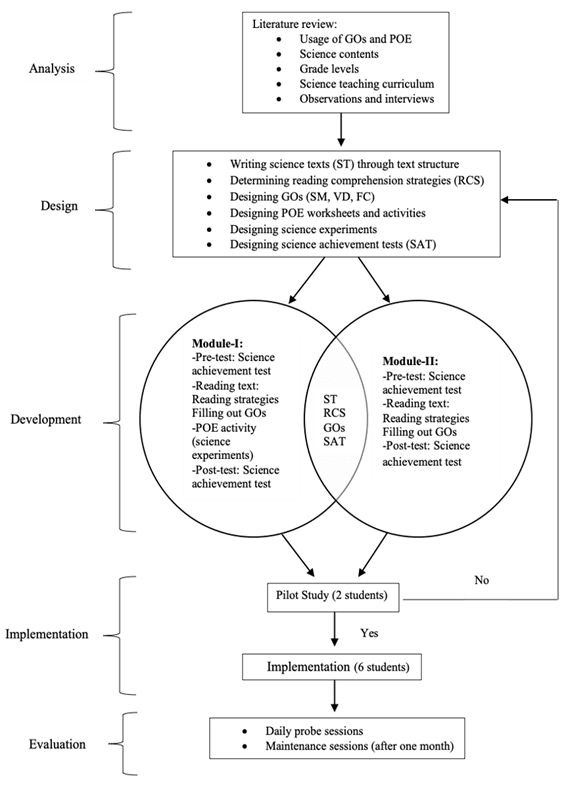
\includegraphics[width=\linewidth]{images/fig1.png}
    \caption{Development of Module-I (GOs+POE) and Module-II (GOs)}
\end{figure}

\subsubsection*{Assessments}
Six unique science achievement tests were created including nine questions to measure student performance across the six science contents. Each individual test targeted to assess equal three skills in the following: (a) giving the specific description of the concept; (b) giving the characteristics of the concept; and (c) giving the examples of the concept from daily life. These skills were selected because each science text created with the same number of steps to provide a same construction for the texts and required similar types of questions to be completed (e.g., multiple-choices, true-false, and filling the blank)—thus ensuring reliability across six assessment tests. All questions were identical in content and format to those covered in the Module-I and Module-II instruction lessons. End of each session of each concept, assessment test was given consisted of nine questions covering each of the three skills within each concept. Science and special education professors established the content validity of the tests and one experienced science teacher checked the test for clarity and appropriateness for student level. Parallel test reliability for the couple of text types is following: Microscopic Organisms and Magnets tests, prepared for the description text type, was .73; Heat \& Temperature and Plant \& Animal Cells tests prepared for the comparison text type was .85; Energy Production and Wastewater Treatment tests, prepared for the sequencing text type, was calculated as .76. These assessment tests were used at the baseline, end of the daily interventions, and in the maintenance sessions one month after the implementation. 

\subsection*{Experimental Design}
A single-subject adapted alternating treatments design (AATD) with baseline, intervention, follow-up and maintenance sessions was used to compare the effectiveness and efficiency of Module-I and Module-II on the science achievement of students with LD in science. The researchers followed the single case design standards of What Works Clearinghouse (WWC) with an AATD, with each student serving as his/her own control, and each data point after intervention served as a replication of a treatment effect (Gast \& Ledford, 2014). In order to make decisions about whether the design is appropriate for evaluating interventions, standards for evaluation of design, conducting visual analysis, and effect-size estimation were considered for enhancing internal and external validity. The standards were met with (a) manipulating independent variables (e.g., Module-I and II interventions) systematically in morning and afternoon sessions, (b) measuring variables systematically over time with two assessors, (c) demonstrating an intervention effects of Module-I and II with three repetition with three group of students (e.g., part-1, part-2, part-3), (d) collecting data at least three time points in a phase for stabilization (e.g., four time points for baseline phase,  three time points for follow-up phase), (e) alternating sequence of the modules with at least five repetitions, (f) considering six outcome-measure (e.g., level, trend, variability, immediacy of effect, overlap, and consistency data patterns), (g) including effect size estimation statistics for consistent results (WWC, 2008). 

\subsection*{Procedures}
Research design basically consists of baseline, intervention, and maintenance phases. Following four sessions of baseline, at least five intervention sessions of Module-I and Module-II each were alternated to assess student performance on science achievement test questions. Following meeting criteria, three follow-up sessions were conducted for each treatment condition. After completing of intervention sessions one-month later data was collected to examine for maintenance.

\subsubsection*{Baseline Phase}
Students were assessed on their ability to solve science achievement test questions without any prior instruction and received no prompting from researchers across the four baseline sessions. Each baseline session involved students completing nine science achievement test questions via paper and pencil. Baseline data was collected four consecutive days for each participant. All baseline sessions were not implemented concurrently to all students. However, baseline data was collected concurrently from the students who are in the same part (part-1, part-2, part-3).  Students moved out of baseline when they had completed four baseline sessions and data were stable.

\subsubsection*{Intervention Phase}
Each student randomly alternated between two treatment conditions: receiving instruction via Module-I: POE argument-based inquiry embedded with GOs or via Module-II: GOs procedure from principal researcher. Module-I and Module-II teaching sessions began for students after four baseline sessions when data stabilized. There were at least two hours between Module-I and Module-II teaching session. As an example, while intervention Module-I was implemented in the morning and intervention Module-II in afternoon, with alternating interventions implemented over multiple days. Thus, carry-over effect was taken under control for Module-I and Module-II. Additionally, six different science contents were selected to avoid carry-over effect.  Modules were implemented respectively to part-1(Ata and Aras), part-2 (Izel and Mert), and part-3 (Yunus and Ayla) students. After part-1 students’ interventions, principal investigator started to interventions for part-2 students. Part-3 students attended to interventions lastly. While teaching sessions of Module-I includes six basic steps, Module-II includes three steps (refer to Table 2 for intervention steps of Module-I and Module-II lessons).

\textbf{Module-I Treatment Condition.} In this module GOs were enhanced with POE argument-based inquiry procedure. Each teaching session consisted of six basic steps. First, students answered the science achievement test questions (pre-test). Second, they began to read the science texts using reading comprehension strategies to fill out the GOs for analyzing and summarizing of the science text. Third, students started to POE activity by predicting the answers of the science experiments’ questions related to big ideas of texts. In this step they gave a scientific claim about the questions of text concepts. Fourth, they started experiments and observed results to evaluate their arguments. Directions and experiment materials of the experiment were given to students in the POE sheet. Fifth, they explained differences between their prediction and observation by using experiment results, tables, schemas, and charts. In this step they compared their claims and results of the experiments by using their evidence to explain whether their claims or arguments are accurate in the last section of the POE sheet. Finally, they answered the nine science achievement test questions on the assessment sheet (post-test). If the student solved 85\% of the questions correctly, intervention was considered successful, and the student moved onto the follow-up session. This cutoff (85\%) was determined based on previous study results in literature (Knight et al., 2013). Follow-up sessions were conducted just like teaching sessions until data stabilized. To following students’ highest calculated percent accuracy average, follow-up data were collected for at least three sessions. 

\textbf{Module-II Treatment Condition.} In this treatment condition, students followed three steps for each session: (1) answering the science achievement test questions (pre-test), (2) reading text using reading comprehension strategies to fill out GOs for analyzing and summarizing of the text, and (3) answering the questions on the assessment sheet (post-test). If the student solved 85\% of the questions correctly, intervention was considered successful, and the student moved onto the follow-up session. Follow-up sessions were conducted just like intervention sessions until data stabilized. Follow-up data was collected for at least three sessions. 

\subsection*{Maintenance Phase}
Maintenance probes were conducted one-month later post the intervention sessions for both Module-I and Module-II conditions. Students were given a similar assessment test used during baseline and intervention phases. Data was collected in one session with each student assessed as to whether they could generalize the acquired skills across different settings. 

\subsection*{Reliability}
Reliability data was collected through treatment integrity and inter-observer agreement for at least 30\% of each experimental condition with sessions in each condition selected randomly. For the treatment integrity, two special education teachers who were familiar with the interventions collected reliability data. A separate Treatment Integrity Checklist for Module-I and Module-II was developed - TICM-I and TICM-II. These checklists were filled out by special education teachers during intervention sessions for both modules. Each component was assessed on a 2-point Likert type scale of 1 (observed) and 0 (not observed (N/O). Treatment integrity is acceptable for intervention phase for all students in Module-I (\textit{M}= 94.1\%; range= 88.5-100) and in Module-II (\textit{M}= 96.2\%; range= 92.2-100). Inter-observer agreement (IOA) was recorded on a student’s ability to complete tasks for Module-I and Module-II (\textit{M}= 98.1\%; range= 88.8-100). An independent observer and principal researcher coded videotaped sessions independently.

\begin{table*}[th]
\caption{General instructional steps of Module-I and Module-II conditions}
\begin{tabular}{ll}
\hline
\textbf{MODULE-I:} GOs+POE Argument-Based Inquiry & \textbf{MODULE-II:} Graphic Organizers (GOs) \\ \hline
\underline{\textit{Pre-test:}} & \underline{\textit{Pre-test:}} \\
Science Reading Comprehension Test & Science Reading Comprehension Test \\
\underline{\textit{Reading Activity:}} & \underline{\textit{Reading Activity:}} \\
\begin{itemize}[noitemsep, topsep=0pt]
    \item Reading Text (e.g., microscopic org.)
    \item Glance down text quickly
    \item Underline unknown words
    \item Determine purpose of reading 
    \item Read text outload
    \item Underline important sentence
\end{itemize} &
\begin{itemize}[noitemsep, topsep=0pt]
    \item Reading Text (e.g., magnets)
    \item Glance down text quickly
    \item Underline unknown words
    \item Determine purpose of reading 
    \item Read text outload
    \item Underline important sentence
\end{itemize} \\
\underline{\textit{Using GOs:}} & \underline{\textit{Using GOs:}} \\
\begin{itemize}[noitemsep, topsep=0pt]
    \item Analyzing of text using first GO (e.g., spider map)
    \item Summarizing of text using second GO (e.g., spider map)
\end{itemize} &
\begin{itemize}[noitemsep, topsep=0pt]
    \item Analyzing of text using first GO (e.g., spider map)
    \item Summarizing of text using second GO (e.g., spider map)
\end{itemize} \\
\underline{\textit{POE Activity:}} & \\
\begin{itemize}[noitemsep, topsep=0pt]
    \item \textit{Predicting} answers of experiments’ questions
    \item \textit{Observing} experiments
    \item \textit{Explaining} difference between predictions and observations (using tables, schemas, charts etc.)
\end{itemize} & \\
\underline{\textit{Post-test:}} & \underline{\textit{Post-test:}} \\
Science Reading Comprehension Test & Science Reading Comprehension Test \\ \hline
\end{tabular}
\end{table*}

\subsection*{Data Analysis}
Effectiveness, efficiency and social validity data were collected to show output of the both instructional modules. To analyze each student’s effectiveness data, the researchers completed visual analysis, an overlap, and effect size measure. Visual analysis assessed considering level, trend, and stability between phases for each student’s graphed data. The percentage of correct responses was calculated using the formula “(Number of correct responses/ Total number of questions) x 100” and transposed into a graph. For an overlap and effect size measure, the researchers calculated Tau-\textit{U}, a nonparametric statistical measure of effect size obtained by combining the non-overlap data between two phases with the trend within the intervention phase (Parker et al., 2011). Tau-\textit{}U is reported as a number ranging from 0 to 1 and interpretation of effect sizes as follows based on the guidelines reported by Ferguson (2009) as follows: minimal effect sizes are .20 to .49, moderate effect sizes are .50 to .79, and strong effect sizes are .80 and above. The Tau-\textit{U} estimates were calculated using online calculators (Vannest et al., 2016). For the efficiency, data was collected about the number of training sessions to criterion, sessions achieved 100\% accuracy, number of correct responses in maintenance session, and training time (duration) for both instructional conditions. When the children met the criteria, the efficiency data was analyzed descriptively. For social validity, A Social Validity Interview Form (SVIF) including six open-ended questions was used to collect data. SVIF were sent to five experts for to examine face validity with the form modified accordingly. The SVIF was designed by researchers to reveal (a) what problems had been caused reading comprehension failure, (b) what was the more beneficial and helpful thing to understand science texts, (c) what were the contributions of graphic organizers for reading science texts, (d) what comprehension skill was influence most by both modules, (e) what were the most liked and least liked part of the study, and (f) which strategy was most useful in learning the science content. Interviews were conducted individually after the interventions and took 15-20 mins. Social validity data were transcribed verbatim and analyzed descriptively by principal researcher.

\section*{RESULTS}
\subsection*{Effectiveness of Module-I and Module-II Interventions}
See Figures 2 through 4 for more information on individual students’ percentages of correct responses during baseline, intervention, and maintenance sessions across the two conditions (GOs+POE and GOs). Figure 2 presents first part students’ (Ata and Aras) science achievements scores on the contexts of “Microscopic Organisms” and “Magnetism”. Figure 3 displays second part students’ (Izel and Mert) scores on “Heat \& Temperature” and “Plant \& Animal Cells”. Figure 4 provides third part students’ (Yunus and Ayla) science scores on “Wastewater Treatment Process” and “Energy Production”. Once they began interventions with Module-I and Module-II, the levels and trends of their data changed dramatically, and they reached the criterion by performing with 85.0\% or greater accuracy after the interventions. 

Students initially performed stable responses during baseline sessions, resulting in average score ranging from 30.3\% to 56\% for Module-I, and from 19.3\% to 52.3\% for Module-II conditions. There was no trend (variability) in the baseline sessions for Ata, Aras, Mert, Yunus, and Ayla. However, Izel’s responses showed a decreasing trend. When levels of their data across baseline and intervention conditions were compared, significant increases were noted in both intervention conditions for all students. Within intervention, their scores for both treatments rose above baseline levels, illustrating an abrupt change in level between phases (refer to Figure 2, Figure 3, and Figure 4). 

For the results of Module-I conditions, Ata earned a total average of 89\% (range = 78 to 100), Aras earned 86.8\% (range = 56 to 100), Izel earned a total average of 81.2\% (range = 56 to 100), Mert earned a total average of 77.6\% (range = 44.4 to 100), Yunus earned a total average of 90.8\% (range = 56 to 100), and Ayla reached a total average of 92.6\% (range = 78 to 100).  In Module-II conditions, Ata earned a total average of 87.2\% (range= 56 to 100), Aras earned a total average of 85.3\% (range= 56 to 100), Izel reached a total average of 71.6\% (range= 33.3 to 100), Mert earned a total average of 77.8\% (range= 44.4 to 89), Yunus earned total average of 81.6\% (range= 56 to 100) accuracy, and Ayla earned a total average of 85.3\% (range= 67 to 100) accuracy in Module-II condition. An increasing trend was observed during both treatment conditions for all participants. 

\begin{figure}[ht]
    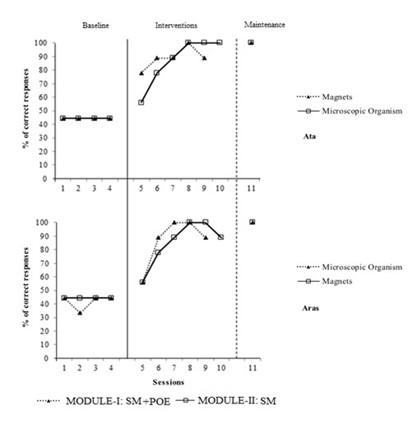
\includegraphics[width=1\linewidth]{images/fig2.jpg}
    \caption{First Part of the Interventions: Comparison of Performances of Ata and Aras} \vspace{1em}
    \textit{Note}. SM= spider map, POE= predicting-observing-explaining
\end{figure}

Both Module-I and Module-II interventions, a three-step follow-up session was made to collect independent performance. In follow-up sessions, all students’ average independence test scores were \textit{M} = 95.6\% (range = 92.6 to 100) in Module-I conditions, and \textit{M} = 93.2\% (range = 89 to 100). All six participants maintained improved levels of science achievement \textit{M} = 100\% for Module-I condition after one-month after instruction ended. While three students (Ata, Aras, Mert) maintained their science achievement \textit{M} = 96.3 (range = 89 to 100) above criteria in Module-II conditions, rest of three students (Izel, Yunus, Ayla) maintained their science achievement \textit{M} = 74.3 (range = 67 to 78) under the criteria of 85\%. Visual analysis indicated all students with LD appeared to benefit from instructions. 

\begin{figure}[ht]
    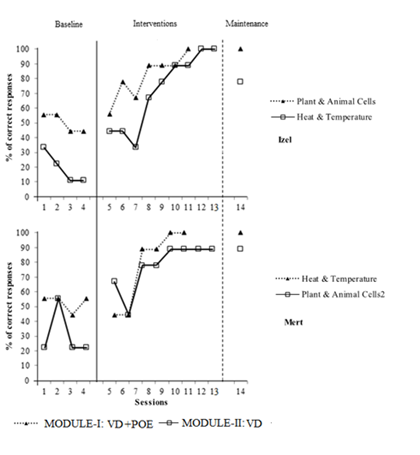
\includegraphics[width=1\linewidth]{images/fig3.png}
    \caption{Second Part of the Interventions: Comparison of Performances of Izel and Mert} \vspace{1em}
    \textit{Note}. SM= spider map, POE= predicting-observing-explaining
\end{figure}

We calculated Tau-\textit{U} using \url{http://www.singlecaseresearch.org/calculators/tau-u} using raw scores. This analysis indicated that science achievements of Ata and Aras improved substantially after instructions (τ = 1, \textit{p} < .05, 90\% confidence interval [CI] [0.26, 1]) for Module-I, and (τ = 1, \textit{p} < .05, 90\% confidence interval [CI] [0.29, 1]) for Module-II. Consistent with our findings from visual analysis, Tau-\textit{U} analysis of raw scores supported that Izel demonstrated significant improvement after instruction (τ = .93 p < .05, 95\% CI [0.31, 1]) for Module-I, and (τ = .97 \textit{p} < .05, 95\% CI [0.38, 1]) for Module-II. Mert performed better achievement in Module-I condition (τ = .83 \textit{p} < .05, 95\% CI [0.19, 1]) than Module-II condition (τ = .78 p < .05, 95\% CI [0.18, 1]). Upon visual analysis, we found that Tau-\textit{U} analysis demonstrated that Yunus and Ayla made substantial improvement on the science achievement tests after instruction in Module-I condition (τ = 1 \textit{p} < .05, 95\% CI [0.36, 1]). Yunus (τ = .95 \textit{p} < .05, 95\% CI [0.23, 1]) and Ayla (τ = 1 p < .05, 95\% CI [0.32, 1]) showed improvement in Module-II conditions.

\begin{figure}[ht]
    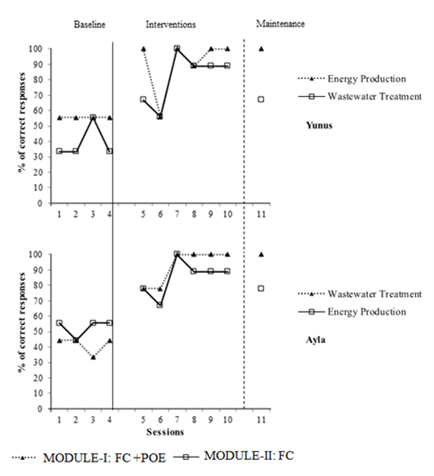
\includegraphics[width=1\linewidth]{images/fig4.png}
    \caption{Third Part of the Interventions: Comparison of Performances of Yunus and Ayla} \vspace{1em}
    \textit{Note}. SM= spider map, POE= predicting-observing-explaining
\end{figure}

\subsection*{Efficiency of Module-I and Module-II Interventions}
Efficiency data, the number of intervention sessions to criterion, the number of sessions performed 100\% accuracy, the number correct responses in the maintenance session, and total training time to criterion—for Module-I and Module-II intervention conditions (see in Table 3). 

\begin{table*}[th]
\caption{Efficiency Results of Module-I and Module-II}
\begin{tabular}{ccccccc}
\hline
\textbf{Student} & \textbf{Independent variables} & \textbf{Dependent variables} & \textbf{Number of IS through criterion} & \textbf{100\% Accuracy} & \textbf{Correct responses in MS} & \textbf{Duration (h:min:s)} \\ \hline
Ata & Module-I: SM+POE & Magnets & 2 & 2 & 9 & 00:50:29 \\
 & Module-II: SM & Microscopic Organisms & 3 & 4 & 9 & 00:48:55 \\
Aras & Module-I: SM+POE & Microscopic Organisms & 2 & 3 & 9 & 00:56:54 \\
 & Module-II: SM & Magnets & 3 & 3 & 9 & 00:50:33 \\
Izel & Module-I: VD+POE & Plant \& Animal Cells & 4 & 2 & 9 & 00:60:05 \\
 & Module-II: VD & Heat \& Temperature & 6 & 2 & 7 & 00:51:41 \\
Mert & Module-I: VD+POE & Heat \& Temperature & 3 & 3 & 9 & 00:48:39 \\
 & Module-II: VD & Plant \&Animal Cells & 5 & 0 & 8 & 00:46:26 \\
Yunus & Module-I: FC+POE & Energy Production & 3 & 5 & 9 & 00:46:46 \\
 & Module-II: FC & Wastewater Treatment & 3 & 1 & 6 & 00:36:21 \\
Ayla & Module-I: FC+POE & Wastewater Treatment & 3 & 5 & 9 & 00:40:51 \\
 & Module-II: FC & Energy Production & 3 & 1 & 7 & 00:30:22 \\ \hline
\end{tabular}
\end{table*}

Consistent efficiency findings in favor of one intervention could not be determined across all parameters. Although Module-I seemed to be more efficient across four students in terms of number of intervention session through criterion, it was not replicated with Yunus and Ayla. Their number of intervention sessions are equal (Module-I= 3, Module-II= 3) for both modules. The number of sessions performed with 100\% accuracy was measured by considering intervention and maintenance sessions. While Mert, Yunus, and Ayla achieved 100\% accuracy performance respectively in three, five, and five sessions of Module-I conditions, Ata had less efficient performance in Module-I condition than Module-II. Aras and Izel had equal 100\% accuracy performance in both treatment conditions. When it comes to number of correct responses in the maintenance session, while all students correctly answered all questions one month later in Module-I conditions, only two students answered correctly all questions in Module-II conditions one month later. Total training time (duration of sessions) of Module-II was shorter than Module-I across all students which may suggest that the training time of Module-II was more efficient than Module-I.

\subsection*{Social Validity Findings}
The six students were asked about the social validity of both interventions, and specifically which method of instruction they preferred for learning - Module-I or Module-II instruction. Social validity data indicated that four students preferred the Module-I instruction best because they thought that POE argument-based inquiry had a specific experiment for each science text to understand better, and two students prefer both Module-I and Module-II instructions. Their answers varied, for example, participant “Aras”, a 13-year-old student, described both instructions were the same expressing “I prefer both. I could understand a text when I read it six or seven times before these instructions.” Participant “Yunus”, a 12-year-old student, agreed with Aras describing his idea a “these two methods supporting each other.” Other participants Ata, Izel, Mert, and Ayla preferred Module-I. Participant “Izel”, a 12-year-old student, preferred the Module-I instruction as it provided more “meaningful learning”. Participant “Mert”, a 12-year-old student, preferred Module-I and stated that he enjoyed because it provided full learning, and it was useful to understand science.” Participant “Ayla”, 13-year-old student, preferred Module-I instruction to meaningful learning and stated that “The funny things stay in my mind more.” 

\section*{DISCUSSION}
The objective of this study was to extend the limited research investigating the effects of GOs enhanced with POE argument-based inquiry (Module-I) and GOs (Module-II) in science teaching for middle school-aged students with LD. In summary, the data revealed that both GOs+POE and GOs procedures were effective in teaching science to students with LD. Even if all six middle school students with LD demonstrated improved performance solving science achievement test questions with both interventions, efficiency and social validity had better outcomes on all dependent variables measured in Module-I procedure (refer to Figure 5). The following conclusions can be drawn on the basis of the data.

\begin{figure}[ht]
    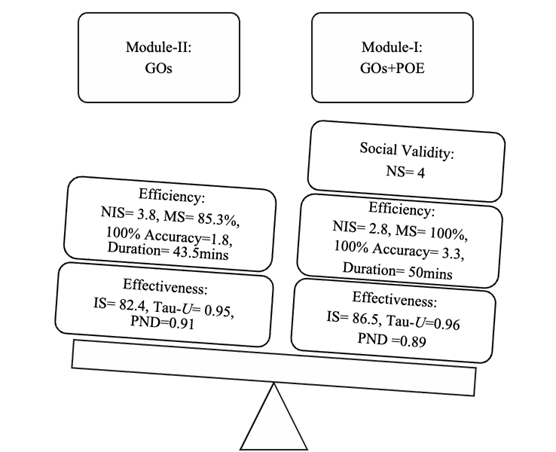
\includegraphics[width=1\linewidth]{images/fig5.png}
    \caption{Summary of Results: Comparison of Module-I and Module-II Conditions} \vspace{1em}
    {\textit{Note}. IS= intervention sessions, NIS= number of intervention session, MS= maintenance session, NS= number of students. For effectiveness, figure shows all students’ mean of IS, Tau-\textit{U}, and PND values. For efficiency, figure includes all students’ average NIS to criterion, average NIS with 100\% accuracy, average MS, and average durations.}
\end{figure}

First, based on the effectiveness data a functional relation was established between the students’ receiving instruction with both Module-I and Module-II procedure and their accuracy performance on science achievement tests. The data are consistent with the findings of previous studies that investigated the effectiveness of GOs (Griffin et al., 2006) and GOs enhanced with POE argument-based inquiry (Bulgren et al., 2014) for teaching this population. The findings of this study enhance the existing literature regarding the effectiveness of GOs and POE. However, to our knowledge, no studies have compared these instructional procedures in teaching science contents. It could thus be started that this study contributes to the current literature by examining the differential effects of both procedures on teaching science to students with LD. Although Tau-\textit{U} effect size measures show both Module-I and Module-II procedures are effective on students’ science achievements in terms of comparison of baseline and intervention sessions, average of test scores (86.5\%) in Module-I was greater than average of test scores (82.4\%) in Module-II. These findings are consistent with the findings of previous studies (Gaddy et al., 2008; Taylor et al., 2018).

Second, analysis of efficiency data resulted that GOs enhanced with POE (Module-I) procedure was more efficient than GOs without POE (Module-II) format in terms of all students’ average number of intervention sessions to criterion (2.8), average number of intervention sessions resulted in 100\% accuracy performance (3.3), and average performance of maintenance sessions (100\%). However, in terms of average duration for both procedure, Module-II was more efficient with 43.5 minutes than Module-I with 50 minutes (see Figure 5). Students maintained their skills after one month and obtained higher scores comparison to baseline for both procedures. While two students (Ata and Aras) showed 100\% accuracy for both intervention conditions, four students (Izel, Mert, Yunus, and Ayla) showed better performance in Module-I than Module-II after one month. There is a one study, especially with GOs supported with argumentation, in which teachers delivered GOs with argumentation intervention. Findings of the study show that the group trained using GOs associated with argumentation strategies had higher academic achievement than the group performed using traditional teaching (Bulgren et al., 2014). 
Third, the findings regarding the social validity of the study showed that all six students responded very positively in general about Module-I. Module-I was preferred by the majority of students more than Module-II. While four students preferred the Module-I instruction, two students prefer both Module-I and Module-II instructions. In order to evaluate the effects of inquiry-based instructions, social validity data were collected from teachers and parents in previous studies (Browder et al., 2012). We need to know students’ idea about inquiry-based instructions whether these methods are useful or not. For this reason, the social validity data of this study enhances the existing literature regarding the collecting data from students.

The results of this study impact the broader field of special education research in two ways. First, our findings support previous literature showing argument-based inquiry to be effective for teaching science to students with LD (Karaer \& Melekoglu, 2020). As a specific form of GOs (spider map, venn diagram, and flow chart) used texts structures accordingly and supported with argument-based inquiry increased students’ reading comprehension skills related to middle school science curricula to this population. Second, the use of POE argument-based inquiry in our study was shown to be nearly as successful as GOs—an established evidence-based practice for teaching science students with LD (Dexter \& Hughes, 2011). In addition, both strategies allow educators to use visual diagrams and illustrations to aid in the learning process (Cihak \& Bowlin, 2009). Creating visual representations of concepts is identified as an effective representation strategy for meaningful learning for students with LD (Gonsalves \& Krawec, 2014). This suggests that students with LD in science are capable of receiving instruction on middle school science curricula (5, 6, 7 and 8th grade) through GOs such as spider map, flow chart, and venn diagrams. If these GOs are enhanced with argument-based inquiry strategies such as POE, there is potential for students to develop richer understanding of the scientific knowledge. While GOs provide opportunities for creating concept maps to organize knowledge, POE creates a written or oral explanation of the materials (Fiorella \& Mayer, 2015). GOs enhanced with POE argument-based inquiry provides students with multiple options in terms of the reading text materials, summarizing text with GOs and explaining arguments using claim, evidence, and rebuttals depending on experiment’s results. Module-I and Module-II provided students text reading strategies to be used before, during and after reading process to understand text helping them know how to use and when to use these strategies for meaningful learning (Botsas, 2017; Dunlosky et al., 2013). However, Module-I also provides students with the opportunity to learn how to use components of argumentation such as data, evidence, claim, and rebuttal while self-explaining and practicing solving scientific problems related to science text (Taylor et al., 2018). Thus, students can learn writing-to-learn strategies (i.e., students learn about science through writing about science experiences), science literacy (i.e., understanding the content, concepts, and processes of science), and inquiry-based instruction (i.e., collecting data, making claims, testing hypotheses, and providing evidence) (Yore et al., 2003). 

\subsection*{Limitations and Future Directions}
Several points and limitations observed during the study should be underlined. First, this study was limited to teaching six science contents consisted of three type of text structure and GOs to six students with LD. Including a larger number of students with other types and grade levels of disabilities is warranted in the future studies. Second, there is a sample of individual practice of argument-based inquiry using single-subject design in this study. However, this study was limited the interaction between students in small group or whole class discussion providing opportunity to learn how to use components of epistemic tools of inquiry such negotiation, language, dialogue, while self-explaining and practicing solving scientific problems related to science text (Hand et al., 2021). Third, the fact that the same content and type of text structure had not been tried at different grade levels limits making a comparison between the grade levels/age of the students. The studies investigating the effects of strategies such as mapping and explanation used in generative science learning environments on students at different grade levels are insufficient in existing related literature (Brod, 2020). Fourth, in generative learning environments where argument-based inquiry strategies are used, students are expected to make inquiries about the content and produce ideas by making predictions before instruction. For this reason, it is considered more effective to implement the predicting phase before instruction, due to the implementation steps of argument-based inquiry (Hand et al, 2021). In this direction, implementation of POE strategy activities after the science text reading phase in the teaching sessions conducted by the researcher can be considered as a limitation. However, since it did not cause any negative outcomes in the research process, it is thought that it did not affect the findings. Future researchers are advised to implement the predicting phase before reading texts or instruction to increase effectiveness and efficiency of POE argument-based inquiry on student’s achievement. 

This study is comparing the effectiveness and efficiency between GOs enhanced with POE argument-based inquiry and GOs without POE on teaching science. Replication studies can be designed to compare both procedures in different settings (e.g., inclusion settings) to teach different science contents. The students were isolated from their groups, and instruction was provided on a one-on-one basis. Future research should be conducted to examine the effects of embedded instruction in the small group or whole class without pulling out the students.

\subsection*{Ethics Statement}
This study required the ethical approval since it is a human subject research. Ethical approval number is 202106304 giving by Institutional Review Board (IRB)- Behavioral/Social Science Ethics Committee.

\subsection*{Disclosure Statement}
No potential conflict of interest was reported by the author(s).

\end{large}
\clearpage
\section*{REFERENCES}\par 

\leftskip 0.25in
\parindent -0.25in

Ardasheva, Y., Norton-Meier, L., \& Hand, B. (2015). Negotiation, embeddedness, and non-threatening learning environments as themes of science and language convergence for English language learners. \textit{Studies in Science Education, 51}(2), 201-249. \url{https://doi.org/10.1080/03057267.2015.1078019}

Ausubel, D.P. (1960). The use of advance organizer in the learning and retention of meaningful verbal material. \textit{Journal of Educational Psychology, 51}(5), 267-272. 

Bay, M., Staver, J. R., Bryan, T., \& Hale, J. B. (1992). Science instruction for the mildly handicapped: Direct instruction versus discovery teaching. \textit{Journal of research in science teaching, 29}(6), 555-570. \url{https://doi.org/10.1002/tea.3660290605}

Botsas, G. (2017). Differences in strategy use in the reading comprehension of narrative and science texts among students with and without learning disabilities. \textit{Learning Disabilities: A Contemporary Journal, 15}(1), 139- 162.

Breitwiest, J. \& Brod, G. (2021). Cognitive prerequisites for generative learning: Why some learning strategies are more effective than others. \textit{Child development, 92}(1), 256-272. \url{https://doi.org/10.1111/cdev.13393}

Brod, G. (2020). Generative learning: Which strategies for what age? \textit{Educational Psychology Review, 33}, 1295-1318. \url{https://doi.org/10.1007/s10648-020-09571-9}

Browder, D. M., Trela, K., Courtade, G. R., Jimenez, B. A., Knight, V., \& Flowers, C. (2012). Teaching mathematics and science standards to students with moderate and severe developmental disabilities. \textit{The Journal of Special Education, 46}(1), 26-35. \url{https://doi.org/10.1177/0022466910369942}

Bulgren, J. A., Ellis, J. D., \& Marquis, J. G. (2014). The use and effectiveness of an argumentation and evaluation intervention in science classes. \textit{Journal of Science Education and Technology, 23}(1), 82-97. \url{https://doi.org/10.1007/s10956-013-9452-x}

 Cihak, D. F., \& Bowlin, T. (2009). Using video modeling via handheld computers to improve geometry skills for high school students with learning disabilities. \textit{Journal of Special Education Technology, 24}(4), 17–29. \url{https://doi.org/10.1177/016264340902400402}
 
Dexter, D. D., \& Hughes, C. A. (2011). Graphic organizers and students with learning disabilities: A meta-analysis. \textit{Learning Disability Quarterly, 34}(1), 51-72. \url{https://doi.org/10.1177/073194871103400104}

Diakidoy, I. N., Ioannou, M. C., \& Christodoulou, S. A. (2017). Reading argumentative texts: comprehension and evaluation goals and outcomes. \textit{Reading and Writing, 30}(9), 1869–1890. \url{https://doi.org/10.1007/s11145-017-9757-x}

Dunlosky, J., Rawson, K. A., Marsh, E. J., Nathan, M. J., \& Willingham, D. T. (2013). Improving students’ learning with effective learning techniques: promising direction from cognitive and educational psychology. \textit{Psychological Science and the Public Interest, 14}(1), 4–58. \url{https://doi.org/10.1177/1529100612453266}

Ferguson, C. J. (2009). An effect size primer: A guide for clinicians and researchers. \textit{Professional Psychology: Research and Practice, 40}, 532–538. \url{https://psycnet.apa.org/doi/10.1037/14805-020}

Fiorella, L., \& Mayer, R. E. (2015). \textit{Learning as a generative activity: Eight learning strategies that promote understanding}. Cambridge University Press. 

Fiorella, L., \& Mayer, R. E. (2016). Eight ways to promote generative learning. \textit{Educational Psychology Review, 28}(4), 717–741. \url{https://doi.org/10.1007/s10648-015-9348-9}

Gaddy, S. A., Bakken, J. B., \& Fulk, B. M. (2008). The effects of teaching text-structure strategies to postsecondary students with learning disabilities to improve their reading comprehension on expository science text passages. \textit{Journal of Postsecondary Education and Disability, 20}(2), 100-119.

Gast, D. L., \& Ledford, J. R. (2014). \textit{Single case research methodology: Applications in special education and behavioral sciences}. Routledge.

Gonsalves, N., \& Krawec, J. (2014). Using number lines to solve math word problems: A strategy for students with learning disabilities. \textit{Learning Disabilities Research \& Practice, 29}(4), 160-170. \url{https://doi.org/10.1111/ldrp.12042}

Griffin, C. C., Simmons, D. C., \& Kameenui, E. J. (2006). Investigating the effectiveness of graphic organizer instruction on the comprehension and recall of science content by students with learning disabilities. \textit{Journal of Reading, Writing \& Learning Disabilities, 7}, 355-376. \url{https://doi.org/10.1080/0748763910070407}

Hand, B., Chen, Y. C., \& Suh, J. K. (2021). Does a knowledge generation approach to learning benefit students? A systematic review of research on the science writing heuristic approach. \textit{Educational Psychology Review, 33}(2), 535–577. \url{https://doi.org/10.1007/s10648-020-09550-0}

Iordanou, K., \& Constantinou, C. P. (2014). Developing pre-service teachers’ evidence-based argumentation skills on socio-scientific issues. Learning \& Instruction, 34, 42–57. \url{https://doi.org/10.1016/j.learninstruc.2014.07.004}

Karaer, G., \& Melekoglu, M. A. (2020). Review of studies on teaching science to students with specific learning disabilities. \textit{Ankara University Faculty of Educational Sciences Journal of Special Education, 21}(4), 789-818. \url{http://doi.org/10.21565/ozelegitimdergisi.532903}

Karaer, G., Hwang, J., Chanlen, N., \& Hand, B. (2024a). Longitudinal study examining immersing students with IEPs in argument-based inquiry to improve the learning of science. \textit{International Journal of Science Education}, 1-20.

Karaer, G., Hand, B., \& French, B. F. (2024b). Examining the impact of science writing heuristic (SWH) approach on development of critical thinking, science and language skills of students with and without disabilities. \textit{Thinking Skills and Creativity, 51}, 101443.

Knight, V. F., Spooner, F., Browder, D. M., Smith, B. R., \& Wood, C. L. (2013). Using systematic instruction and graphic organizers to teach science concepts to students with autism spectrum disorders and intellectual disability. \textit{Focus on autism and other developmental disabilities, 28}(2), 115-126. \url{https://doi.org/10.1177/1088357612475301}

Lin, T., Horng, R., \& Anderson, R. C. (2014). Effects of argument scaffolding and source credibility on science text comprehension. The Journal of Experimental Education, 82(2), 264-282. \url{https://doi.org/10.1080/00220973.2013.769423}

Lynch, S., Taymans, J., Watson, W. A., Ochsendorf, R. J., Pyke, C., \& Szesze, M. J. (2007). Effectiveness of a highly rated science curriculum unit for students with disabilities in general education classrooms. \textit{Exceptional Children, 73}(2), 202-223. \url{https://doi.org/10.1177/001440290707300205}

McDermott, M. A., \& Hand, B. (2013). The impact of embedding multiple modes of representation within writing tasks on high school students’ chemistry understanding. \textit{Instructional Science, 41}(1), 217–246. \url{https://doi.org/10.1007/s11251-012-9225-6} 

Meyer, B. J. F. (1984). Text dimensions and cognitive processing. In H. Mandl, N. Stein, \& T. Trabasso (Eds.), \textit{Learning and understanding texts} (pp. 3–47). Erlbaum.

National Center for Education Statistics. (2019). National assessment of educational progress report card: Science. \url{https://www.nationsreportcard.gov/science/nation/groups/?grade=4,8,12}. 

NGSS Lead States. (2013). Next generation science standards: for states, by states. Washington, DC: The National Academy Press. 
Nussbaum, E. M. (2008). Using argumentation Vee diagrams (AVDs) for promoting argument counter argument integration in reflective writing. \textit{Journal of Educational Psychology, 100}(3), 549–565. \url{https://doi.org/10.1037/0022-0663.100.3.549}

Olson, J. L., \& Platt, J. C. (2004). \textit{Teaching children and adolescents with special needs}. Merrill.

Osborne, J., Erduran, S., \& Simon, S. (2004). Enhancing the quality of argumentation in school science. \textit{Journal of research in science teaching, 41}(10), 994-1020. https://doi.org/10.1002/tea.20035

Parker, R. I., Vannest, K. J., Davis, J. L., \& Sauber, S. B. (2011). Combining nonoverlap and trend for single-case research: Tau-U. \textit{Behavior Therapy, 42}(2), 284–299. \url{https://doi.org/10.1016/j.beth.2010.08.006}

Ritchie, D., \& Wolkl, C. (2000). Effectiveness of two generative learning strategies in the science classroom. \textit{School Science and Mathematics, 2}, 83-89. \url{https://doi.org/10.1111/j.1949-8594.2000.tb17240.x}

Rizzo, K. L., \& Taylor, J. C. (2016). Effects of inquiry-based instruction on science achievement for students with disabilities: An analysis of the literature. \textit{Journal of Science Education for Students with Disabilities, 19}(1), 2-16.

Sak, U., Bal Sezerel, B., Ayas, B., Tokmak, F., Ozdemir, N., Demirel-Gurbuz, S., \& Opengin, E. (2016). \textit{Anadolu-sak intelligence scale} (ASIS) practitioner book. Anadolu University UYEP Center. 

Scruggs, T. E., \& Mastropieri, M. A. (2007). Science learning in special education: The case for constructed versus instructed learning. \textit{Exceptionality, 15}(2), 57-74. \url{https://doi.org/10.1080/09362830701294144}

Seels, B., \& Glasgow, Z. (1998). \textit{Making instructional design decisions} (2nd ed.). Merrill/Prentice Hall. 

Simmons, D. C., Griffin, C. C., \& Kameenui, E. J. (1988). Effects of teacher constructed pre- and post-graphic organizer instruction on sixth-grade science students' comprehension and recall. \textit{Journal of Educational Research, 82}(1), 15-21.

Singleton, S. M., \& Filce, H. G. (2015). Graphic organizers for secondary students with learning disabilities. \textit{Teaching Exceptional Children, 48}(2), 110-117. \url{https://doi.org/10.1177/0040059915605799}

Tabachnick, B. G., \& Fidell, L. S. (2007). \textit{Experimental designs using ANOVA}. Belmont.

Taylor, T. J., et al. (2018). Using argument-based science inquiry to improve science achievement for students with disabilities in inclusive classrooms. \textit{Journal of Science Education, 21}(1), 1-14.

Therrien, W. J., Taylor, J. C., Hosp, J. L., Kaldenberg, E. R., \& Gorsh, J. (2011). Science instruction for students with learning disabilities: a meta-analysis. \textit{Learning Disabilities Research \& Practice, 26}(4), 188-203. \url{https://doi.org/10.1111/j.1540-5826.2011.00340.x}

Vannest, K.J., Parker, R.I., Gonen, O., \& Adiguzel, T. (2016). \textit{Single Case Research: web-based calculators for SCR analysis} (Version 2.0) [Web-based application]. College station. singlecaseresearch.org

What Works Clearinghouse. (2008). \textit{Procedures and standards handbook} (version 2.0). Retrieved July 10, 2009, from \url{http://ies.ed.gov/ncee/wwc/references/idocviewer/doc.aspx?docid=19&tocid=1} 

Yore, L., Bisanz, G. L., \& Hand, B. M. (2003). Examining the literacy component of science literacy: 25 years of language arts and science research. \textit{International Journal of Science Education, 25}(6), 689-725. \url{https://doi.org/10.1080/09500690305018}

\end{document}
